\documentclass[11pt]{article}

\usepackage[lmargin=0.75in, rmargin=1in, tmargin=1.25in, bmargin=1in]{geometry}
\usepackage[english]{babel}
\usepackage[utf8]{inputenc}

\usepackage{amsfonts}
\usepackage{amsmath}
\usepackage{bm}
\usepackage{booktabs}
\usepackage[labelsep=period]{caption}
\usepackage{enumitem}
\usepackage{fancyhdr}
\usepackage{graphicx}
\usepackage{lastpage}
\usepackage{listings}
\usepackage[svgnames]{xcolor}

% For formatting C++ code listings ---------------------------
\lstdefinestyle{customCpp}{
    language=C++,
    keywordstyle=\color{RoyalBlue},
    basicstyle=\footnotesize\ttfamily,
    commentstyle=\color{Green}\ttfamily,
    rulecolor=\color{black},
    numbers=left,
    numberstyle=\tiny\color{gray},
    stepnumber=1,
    numbersep=8pt,
    showstringspaces=false,
    breaklines=true,
    frame = tb,
    belowcaptionskip=5pt,
    belowskip=3em,
    gobble=10,
}

% For turning enumerated lists into Problem titles --------------
\renewcommand{\labelenumi}{\textbf{Problem \arabic{enumi}}}
\renewcommand{\labelenumii}{(\alph{enumii})}

% Enumerated list indents:
% Problems:    [leftmargin=0.9in]
% Subproblems: [leftmargin=0.3in]


% Document Details ----------------------------------------------
\author{Eli Case}
\title{CAAM 420/520 -- Homework 2}
\date{February, 17, 2023}
\makeatletter


% Setup headers -------------------------------------------------
\pagestyle{fancy}
\fancyhf{} % Clear the headers and footers
\lhead{\@author}
\chead{\@title}
\rhead{\@date}
\cfoot{Page \thepage\ of \pageref{LastPage}}
\setlength{\headheight}{15pt}
\setlength{\headsep}{20pt}

\fancypagestyle{plain}{
	\fancyhf{}
	\setlength{\headheight}{15pt}
	\setlength{\headsep}{0pt}
	\renewcommand{\headrulewidth}{0pt}
	\cfoot{\vspace{2mm}Page \thepage\ of \pageref{LastPage}}
}


\begin{document}
\flushleft
\thispagestyle{plain}
To: Christina Taylor

From: \@author

Date: \@date

Subject: \@title

\makeatother
\medskip
\hrule
\medskip

\begin{enumerate}[leftmargin=0.9in]
\item % Problem 1

   \begin{enumerate}[leftmargin=0.3in]

      \item If we use the domain decomposition shown in Figure 1, we cannot parallelize the problem because of the order dependency present when using a backward finite difference stencil. With the given domain decomposition, the threads will have to execute sequentially, as thread 1 cannot execute before thread 0, thread 2 cannot execute before thread 1, etc. Thus, we will be computing the problem serially with the additional overhead of setting up the parallelization, meaning we would want to change the domain decomposition to be able to execute the problem in parallel, while preserving the order-dependency of the problem.

      \item We can begin with the formula for the time to process the spin up region, $T_{full}$.
        \begin{equation}
           T_{full} = N_w(T_s + n_bT_p)
        \end{equation}
        To determine when the synchronization time contributes more to the total spin-up time than the computation time, we can construct the following inequality.
        \begin{equation}
           N_wT_s > N_wn_bT_p 
        \end{equation}
        Reducing this inequality, we have the following.
        \begin{align*}
          T_s &> n_bT_p \\
          n_b &< \frac{T_s}{T_p}
        \end{align*}
        Thus, from above, we have that synchronization contributes more time to $T_{full}$ when the number of elements per block, $n_b$, is less than the ratio of synchronization time to computation time per node, $\frac{T_s}{T_p}$. While smaller blocks provide better parallelization by reducing the spin-up and spin-down time, the cost of synchronization limits how small the block sizes can be, since blocks that are too small cause more spin-up time to be spent on synchronization, rather than computation. 
 
   \end{enumerate} % End of Problem 1 subpoints

 \item %Problem 2

   \begin{enumerate}[leftmargin=0.3in]
     \setcounter{enumii}{1}
     \item
       The overall number of blocks requiring computation is $N_x N_y$. We can compute the number of blocks in the spin-up and spin-down regions, {\fontfamily{cmtt}\selectfont blocks\_spin} as follows.
       \begin{equation}
         \text{{\fontfamily{cmtt}\selectfont block\_spin}} = 2(N_T - 1)!
       \end{equation}

       Similarly, the number of blocks fully parallel region, {\fontfamily{cmtt}\selectfont block\_parallel}, is as shown below.
      \begin{equation}
        \text{{\fontfamily{cmtt}\selectfont block\_parallel}} = N_x N_y - 2(N_T - 1)!
      \end{equation}

      If we assume every block takes the same amount of time to process and synchronize, we can write the ratio of the time spend in the spin-up and spin down region to the fully parallel region as follows.
      \begin{equation}
        \frac{\text{{\fontfamily{cmtt}\selectfont block\_spin}}}{\text{{\fontfamily{cmtt}\selectfont block\_parallel}}} = \frac{2(N_T - 1)!}{N_x N_y - 2(N_T - 1)!}
      \end{equation}

   \newpage
 
 \item

   Below in Figure \ref{fig:1}, we have the computed strongly scaled parallel speed-up plotted across ratios from 1 to 3 for blocks to threads. 
   
   \begin{figure}[!h]
   \centering
   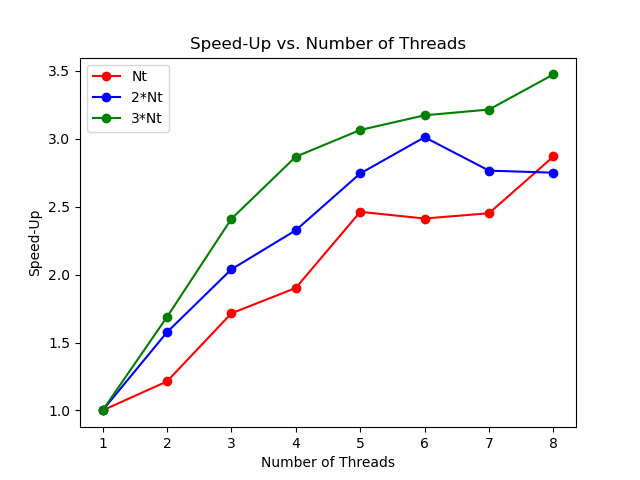
\includegraphics{./figures/speed_up.png}
   \caption{Strong Scaling: Speed-up vs. Number of Threads}
   \label{fig:1}
   \end{figure}

 \end{enumerate} % End of Problem 2 subpoints

\end{enumerate} % End of Problems

\end{document}
